

\section{Setup}
In this section, we describe the process of gathering information regarding
known vulnerabilities (in the form of CVEs) for web applications, designing
and executing tests against web applications of interest, and identifying
the server-side code that was executed as a result of client-side actions.

\subsection{Overview}
The setup for our framework is depicted in
Figure~\ref{fig:debloatingpipeline}. To debloat target applications, we first
collect information about the vulnerabilities of the applications that we
analyze in our study. This information includes the files, functions, and
line numbers where each
vulnerability resides (Step 1, Section~\ref{sec:vulntosourcemapping}). Then,
we simulate usage of the application through a combination of different
techniques (Step 2, Section~\ref{subsec:profiling}). Using a PHP profiler
tool (\texttt{XDebug}), we record the lines, functions, and files, that are
triggered during the simulation (Step 3, Section~\ref{subsec:coverage}).

\begin{figure*}[t]
  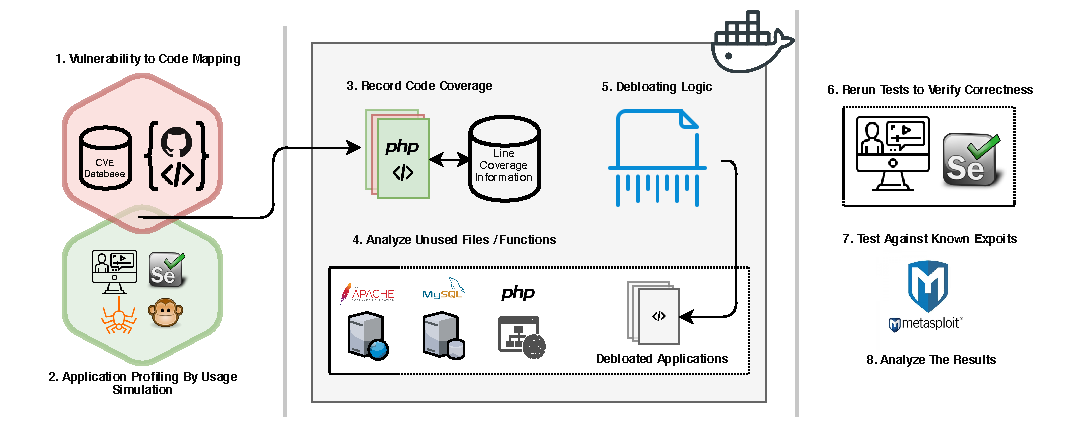
\includegraphics[width=\linewidth]{figures/lim/DebloatingPipeline.pdf}
  \caption{Overview of the architecture of our pipeline for debloating web applications and assessing the effects of different debloating strategies.}
  \label{fig:debloatingpipeline}
\end{figure*}

In the middle part of our pipeline, the debloating engine takes both the
target applications and coverage information to perform debloating at
different levels of granularity, and rewrite parts of the application to
remove unused pieces of code based on the debloating strategy being evaluated
(Steps 4 and 5, Section~\ref{sec:debloating}). Our framework also provides
a complete reporting panel to assist human analysts in understanding which
vulnerabilities can be removed by the present debloating strategies.

Last, we verify the correctness of our debloating process by running
a set of tests against the debloated web applications, and verifying that
no removed piece of code is triggered (Step 5). To this end, we
utilize assertions in place of the removed code blocks. An absence of error
messages from these assertions means that all tests were successfully
completed without triggering any missing server-side code. As a final step of
verification, we also test the debloated applications against a series of
exploits and verify that exploits which
abuse any of the vulnerabilities that were removed as part of the debloating
process, do not succeed (Step 6, Section~\ref{section:metasploit}).

To ease the integration and facilitate the analysis of new web applications, we
adopted a modular architecture that relies on three Docker containers. The
\textit{Application} container hosts our web applications.  The profiler
enabled on its web server is responsible for collecting code-coverage
information. The \textit{Database} container runs a MySQL server that
stores the code-coverage information along with the databases of the tested
applications. Lastly, the \textit{Debloating} container which includes our
debloating logic, analyzes the coverage information and generates debloated
versions of applications. It also provides a reporting panel that indicates
which vulnerabilities are removed in each application after debloating. To add
a new vulnerability, a user simply has to provide the details of the vulnerable
file(s) and line(s).

%In the end, this modular architecture makes the integration of our framework with new web applications and addition of new vulnerabilities seamless.


\subsection{Analyzed web applications}
\label{subsec:webapps}

%\begin{table*}[]
%\centering
%\caption{Analyzed open-source web applications and their corresponding versions.}
%\begin{tabular}{@{}lll@{}}
%%\toprule
%\textbf{Web Application}  & \textbf{Versions} \textit{(Release Date)}                                                                                  & \textbf{Known CVEs} \textit{($\geq$2013)}              \\ \midrule
%\multicolumn{1}{l}{Magento}                          & 1.9.0 \textsubscript{2014-5}, 2.0.5 \textsubscript{2016-4}                                                                             & 10                       \\ \midrule
%\multicolumn{1}{l}{MediaWiki}  & \multicolumn{1}{l}{1.19.1 \textsubscript{2012-06}, 1.21.1 \textsubscript{2013-05}, 1.23.0 \textsubscript{2014-06}, 1.24.0 \textsubscript{2014-11}, 1.28.0 \textsubscript{2016-11}} & \multicolumn{1}{l}{111} \\ \midrule
%\multicolumn{1}{l}{phpMyAdmin} & \multicolumn{1}{l}{4.0.0 \textsubscript{2013-05}, 4.4.0 \textsubscript{2015-04}, 4.6.0 \textsubscript{2016-03}, 4.7.0 \textsubscript{2017-03}}                      & \multicolumn{1}{l}{130} \\ \midrule
%\multicolumn{1}{l}{{Wordpress}}                          & {3.9.0 \textsubscript{2014-4}, 4.0 \textsubscript{2014-9}, 4.2.3 \textsubscript{2015-7}, 4.6 \textsubscript{2016-8}, 4.7 \textsubscript{2016-12}, 4.7.1 \textsubscript{2017-1}}                                                                             & {131}                       \\
%\bottomrule
%\end{tabular}
%\label{table:analyzed_webapps}
%\end{table*}

To understand how the process of debloating increases the security of web
applications, we decided against using toy-like web applications. Instead,
we focused on established open-source applications with millions of users,
and the presence of a sufficient number of known historical vulnerabilities
(in the form of CVEs) to allow us to generalize from them. To this end, we
selected {phpMyAdmin}~\cite{phpmyadmin},
{MediaWiki}~\cite{mediawiki}, {Magento}~\cite{magento}, and WordPress~\cite{wordpress},
which are representative samples of four different types of
web applications namely web-administration tools, wikis, online
shops, and blogging software. Table~\ref{table:analyzed_webapps} shows the versions of these web
applications that we utilized, in order to map CVEs to the location of the
vulnerability in the source code of each application.


%Initially, we study the registered CVEs for a subset of famous open source
%PHP applications. To capture different types of application architectures, we
%cover the following range of categories: \textit{``Web Administration Tools''}
%with phpMyAdmin, \textit{``Wiki''} with MediaWiki and \textit{``Online
%Shops''} with Magento. To map registered CVEs to the vulnerable piece
%of source code for each application, we used a set of versions for each
%application that contain the studied CVEs. These applications are listed
%in Table~\ref{table:analyzed_webapps}.
% We can refer to buildwith stats if we need to reason about why we chose these applications, both usage statistics and registered covers
% Why PHP: https://trends.builtwith.com/framework/programming-language
% Ecommerce: https://trends.builtwith.com/shop

\begin{table}[]
\centering
\caption{Analyzed open-source web applications.}
\scalebox{0.87}{
\begin{tabular}{|l|l|c|}
\hline
\textbf{Web Application} & \textbf{Version}                            & \begin{tabular}[c]{@{}l@{}}\textbf{Known CVEs}\\\hspace{1em}(2013-2019)\end{tabular} \\ \hline
Magento                  & 1.9.0, 2.0.5                                 & 10                                                                     \\ \hline
MediaWiki                & 1.19.1, 1.21.1, 1.24.0, 1.28.0 & 111                                                                    \\ \hline
phpMyAdmin               & 4.0.0, 4.4.0, 4.6.0, 4.7.0     & 130                                                                    \\ \hline
WordPress                & 3.9.0, 4.0, 4.2.3, 4.6, 4.7, 4.7.1  & 131                                                                    \\ \hline
\end{tabular}
}
\label{table:analyzed_webapps}
\end{table}

\subsection{Vulnerability to source-code mapping}
\label{sec:vulntosourcemapping}
To determine whether debloating web applications can actually remove
vulnerabilities, we performed a mapping of known CVEs to the vulnerable lines,
functions, and files, that they exploit in each application. This way, by
looking at an application after debloating, we can determine if the files,
functions, or lines responsible for the vulnerability, are still present or
were removed during the debloating process.


Even though there exist multiple databases listing the current and
historical CVEs of popular software (including the web applications in
question)~\cite{cvedetails,nistgov}, locating the actual source code
containing the vulnerability described in a CVE, is a non-trivial process
which requires careful investigation. In some cases, the right patch can be
discovered because of a direct reference to a CVE in a commit message, or in
a bug report on official public repositories of web applications. For others,
the fix is included within numerous commits that have to be carefully analyzed
to locate the appropriate lines of code. Since a vulnerability can span over
multiple lines, functions, and even multiple files, we record all affected
locations in a database so that this information can be later correlated
with each evaluated application.

%\todo{The following paragraph seems out of place... perhaps something for
%the background section}
%The premise behind debloating is that vulnerabilities exist in parts of a
%program that are never used in specific deployments of interest, and therefore
%can be safely removed (i.e., debloated). This makes the success of debloating
%highly dependent on the usage profile of an application and the location of
%any given vulnerability.
%%In the end, as debloating is based on specific usage profile, some
%%vulnerabilities may be more frequently mitigated than others depending on their
%%location in the source code. If a vulnerability belongs to a feature within
%%the application that is rarely triggered by normal users or that is hidden
%%behind privileged access, they may often be removed from the source code.
%To understand this better, we cam investigate a specific example of critical
%vulnerability. CVE-2016-6620 is a PHP object injection vulnerability that
%affects phpMyAdmin 4.6.0. It has a CVSS score of 9.8 which represents a highly
%severe and critical vulnerability inside phpMyAdmin. It consists of calling
%the PHP \textit{unserialize} function with unsanitized user-supplied data
%which then leads to code execution upon deserialization. This vulnerable
%feature has to be manually enabled by the user and is not part of the
%default configuration of phpMyAdmin. Hence, most usage profiles from real
%users will likely not contain any calls to this PHP \textit{unserialize}
%function, allowing the vulnerable code to be safely removed.


Given the time-consuming nature of mapping CVEs to existing code, for
this study, we limited ourselves to, at most, 20 CVEs per application
of interest.
The complete list of CVEs we mapped for this study can be found in
Table~\ref{table:listofallcves} in the Appendix.
To select these CVEs, we ordered existing vulnerabilities by
their CVSS score (thereby selecting the ones that are the most critical)
and we did not consider vulnerabilities that were reported before 2013. This
focus on fairly recent vulnerabilities (i.e., in the last five years) makes
our results more generalizable to the current state of web applications,
as opposed to quantifying vulnerabilities in source-code which has since
dramatically evolved. Note that, because not all versions of a web application
are vulnerable to all evaluated CVEs, we had to map vulnerabilities
across a number of different versions, as shown in
Table~\ref{table:analyzed_webapps}.



\subsection{Application usage profiling}
\label{subsec:profiling}

Modern web applications provide an incredibly wide range of features and
options to their users. Even though, from a functional perspective, more
features are desirable, from a security perspective, the code that implements
new features may contain new vulnerabilities thereby further expanding
a program's attack surface. In order for a system to be
able to remove code related to unnecessary features, one must first identify
which features are necessary for a target set of users.

Given a usage profile, the goal of our framework is to produce debloated
versions of web applications which maintain the code and features that are
part of that profile but remove the rest. To be as objective as possible with
what features are considered ``necessary,'' we utilize four independent
sources of web application usage: i) online tutorials describing how to use
the applications of interest, ii) web crawlers that autonomously navigate
the application, iii) vulnerability scanners that feed malicious content to the
application, and iv) monkey testing tools that click on random parts of webpages
and type random keystrokes. The combination of all four gives our profiles
both breadth (through the crawler and monkey testing) as well as depth (through
the user following complicated paths while providing expected inputs and the
vulnerability scanner which provides large amounts of malicious inputs trying
to exploit the web application).

%In order to test our pipeline for this study, we created our own usage profile from scratch by using a combination of different automated techniques.
%First, to cover the core features of our tested web applications, we followed online tutorials and wrote Selenium tests based on them.
%This way, we obtain replayable tests that trigger the most essential lines in an application.
%Then, to augment coverage and add easy-to-reach options that are likely to be triggered, we used two additional techniques: spider software that can crawl the pages of the application interface and submit forms, and monkey testing scripts that click on random locations on the screen and type random keystrokes.
%While following the tutorials covers key functionalities within the application, monkey and spider tests add more breadth to our coverage.


%Different users use different parts of web applications, this can be a result of an access restriction model or be based on the need of different users. Specialized applications will have their unique usage profile as studied by [cite the paper that studies usage profile of industry application]. In our model, we simulate a general user that installs the application and uses available online tutorials to find his way through the applications. To that end, we automated the tutorials for our target web applications using selenium, to augment the coverage and add easy to reach options that the users are likely to trigger, we used spider software that would crawl the pages of the website and submit forms in addition to a monkey testing script that would click on random locations on the screen and type random keystrokes. While following the tutorials covers deep functionalities within the application, monkey and spider tests add more breadth to our coverage.

\subsubsection{Tutorials}
\label{sec:tutorials}
To simulate common interactions with an application, we use a popular search
engine to search for the application's name followed by the word ``tutorials''
(e.g., ``phpMyAdmin tutorials'') and follow the tutorials from the first two
pages of search results.

Specifically, we map each tutorial to a Selenium script that allows us to
both execute the same tutorial multiple times and also assess the correctness
of the results (e.g., encode that when we delete a database using phpMyAdmin,
the deleted database is no-longer shown in the list of databases). Note that
this mapping of tutorials to Selenium scripts is yet another time-consuming
process which, occasionally, has to be repeated for different versions of
the same web application. One change in a form field or in a selector can
break the complete flow of a test suite, and we observed a significant number
of cases with slight interface changes between two consecutive versions of
the same application.

Overall, after fine-tuning the scripts for all our tested versions, we obtained
46 tutorials which translated into 302 use cases scripted as Selenium tests
requiring 16,025 lines of code. Given our desire for complete reproducibility
of our results, we include the complete list of tutorials in the Appendix
(Table~\ref{table:listoftutorials}) along with WebArchive links that will
remain available despite potential future domain expirations and linkrot of
the original URLs~\cite{koehler2004longitudinal}.

%Tutorials model the behavior of the vast majority of users who try
%to setup the minimum necessary functionalities of applications and start
%working with them.
%While this approach triggers benign and valid use cases of the applications, it
%does not run code paths that lead to invalid inputs and does not cover the code
%for error handling.

Below, we provide a non-exhaustive list of actions that were part of the followed tutorials of each web application. 
% Full details are available in the actual tutorials and in the Selenium scripts which we will release together with this paper.
\vspace{0.5ex}

\noindent \textbf{Actions covered by phpMyAdmin tutorials:} As a web administration tool, all phpMyAdmin functionality is protected by an authentication mechanism.
We followed the actions described by tutorials when logged in as a root user account with full application access. The Selenium-encoded tutorials cover database operations including creating and dropping databases, filling tables with data, querying, table indexes, and importing/exporting data.
They also include administration tasks such as adding new user accounts, optimizing databases, checking database server status, obtaining performance metrics, and accessing server settings such as variables, charsets, and engines.

\vspace{0.5ex}

\noindent \textbf{Actions covered by MediaWiki tutorials:} MediaWiki provides different features depending on the privileges of the user.
Unauthenticated users can only visit and search pages.
Registered ones can post and edit content while administrators can perform moderation and management operations.
The tutorials that we followed cover all these different use cases.
More specifically, actions coded in our tutorials include authentication, creating and renaming pages, importing and exporting content from the wiki, as well as changing settings such as skins, styles, and formatting options.
%Modifying the navigation menu is a task that can only be performed by an administrator and is also covered by the tutorials. Finally, the tutorials also cover the importing and exporting content from the wiki.

\vspace{0.5ex}

\noindent \textbf{Actions covered by WordPress tutorials:} As a blogging software, WordPress has two distinct entry points, one for normal unauthenticated users to read blogs and post comments, and a separate administration panel accessible to privileged and authenticated users.
WordPress tutorials mostly focus on administrative tasks since normal users have limited abilities. The Selenium-encoded tutorials include actions such as creating a new post using HTML for the content, modifying most post options (ranging from visibility and tags to setting featured images), as well as downloading and changing WordPress themes.
%They cover different settings and include the managing of categories and tags.
For the administration panel, the tutorials include exporting content, setting up user accounts, and uploading media. Finally, the tutorials include the visiting of posts and the posting of comments as well as the management of comments, such as approving them, marking them as spam, and deleting them.
\vspace{0.5ex}

\noindent \textbf{Actions covered by Magento tutorials:} Magento is the largest evaluated web application in terms of source code and has the most features compared to the other applications. Similar to WordPress, the tutorials mostly target administration tasks which include store settings, advanced product search options, order notification via RSS, product pricing, currencies and tax rules, delivery and payment methods, emails and notifications, reviews and ratings and cache control. Some tutorials go in even more details by covering product and stock management, managing customers and groups configurations, modifying the UI, creating pages, and using widgets.
On the customer side, we followed tutorials that included registration of a new account, authentication actions, and purchasing products until checkout.






\subsubsection{Monkey testing}
\label{sec:monkey}
Monkey testing is a method for testing
software where the simulated user sends random clicks and keystrokes to the
target application. This unpredictable behavior can uncover bugs in an
application as it can trigger paths and actions that were not anticipated by
developers. In our case, we use such a technique to trigger additional code,
not covered by tutorials. We observe that this approach adds breadth to the
code-coverage by reaching easy to access features. In addition, by feeding
random keystrokes into forms, monkey testing can bring the application in an
error state thus exercising error-handling pieces of code.

We rely on the stress-testing library called
\texttt{gremlins.js}~\cite{gremlinsjs} in conjunction with the GreaseMonkey
browser extension~\cite{greasemonkey} to inject the library into web
application pages.
%During pilot stages of these experiments, we experimented
%with different configurations for \texttt{gremlins.js} (in terms of its
%combinations of Click, Scroll, Keystroke, and Delays actions) and arrived
%at a configuration that exercised as much as possible of each tested web
%application.
Since this kind of testing can occasionally trigger unwanted actions, we have
to take necessary steps to stop them, e.g., prevent the test from leaving
the web application and visiting external websites. We also want to prevent
\texttt{gremlins.js} from getting trapped on a single page as an unexpected
JavaScript
%\texttt{alert} or \texttt{prompt}
dialogue box or a dead end page can pause our test
execution.  %or the monkey can get stuck on a deadend page.
An additional issue is that of accidentally logging out a web application by
clicking on a logout link. Given that we run monkey-testing under three different
usage profiles (public user, logged-in user, and administrator) we took steps
to avoid accidental logouts. Overall, we perform the following
modifications: i) we remove all links that lead to external pages, ii) we
remove logout buttons for applications that require authentication, iii) we
override the aforementioned JavaScript functions and iv) we set a timeout to
detect when the monkey is stuck and reset it to a known good state. All these
actions are done using injected JavaScript on target pages prior to starting
the \texttt{gremlins.js} library.

To cover a large set of pages from a web application, we run
\texttt{gremlins.js} for 12 hours for each of the test profiles.
To guarantee the reproducibility of our experiment, we choose a fixed seed for
each run that will generate the same sequence of pseudo-random actions.


\subsubsection{Crawling}
Web spiders (also known as crawlers) are a type of bot that follows the
links of a web application and optionally submits forms with predefined
content. Each newly crawled page is added to a database of the application that
the crawler uses to prevent repeated visits to the same pages. For our study,
we use BurpSuite Spider v2.0.14~\cite{burpsuite} to crawl our web
applications. As a result, we augment the application coverage with code paths that were
not triggered, either through the followed tutorials or through monkey testing.

%Our results show that monkey testing and spiders produce different code-coverage and trigger different functionalities within tested applications. Hence, these two methods help us increase the diversity of our usage profiles.
%Hence, this is necessary to include both of these tests.

\subsubsection{Running vulnerability scanners}
Vulnerability scanners are tools that try to detect security flaws in web applications.
%In our case, the scanner increases our code-coverage by reaching unwanted states in the application.
We use BurpSuite Scanner v2.0.14~\cite{burpsuite} based on the URLs extracted by the spider to look for vulnerabilities in headers, URLs and forms.
Notably, the scanner tries different injection mechanisms like SQL injection, XSS, PHP file injection, and path traversal, to trigger errors and reach unwanted states in the application.
The vulnerability scanner goes beyond what the crawler and the monkey cover by modifying headers and URL parameters.
By inspecting the resulting coverage, we observe that each of these four methods result in exercising server-side code that would not have been exercised through the other methods. We quantify this relationship in Section~\ref{section:results}.


\subsection{Recording server-side code-coverage}
\label{subsec:coverage}

Regardless of the method that is used to interact with a web application,
in order to be able to successfully remove unused code (i.e., debloat the web
application), we must be able to
associate client-side requests with server-side code. To record the files
and lines of code that are triggered by user requests, we make use of PHP
profilers.

PHP profilers are available as PHP extensions that modify the PHP engine to
collect code-coverage information. There exist a number of different profilers,
such as, \texttt{XDebug}~\cite{XDebug}, \texttt{phpdbg}~\cite{phpdbg}, and
\texttt{xhprof}~\cite{xhprof} all of which require a similar setup to record
code-coverage. For our framework, we decided to use \texttt{XDebug} as it
is the most mature profiler and is actively maintained.

\subsubsection{Adding coverage support in a web application}

\vspace{1ex}
\noindent\textbf{Connecting a web application to XDebug.}
To be able to perform dynamic analysis and record lines of code
that are triggered by user requests, our framework must add calls
to specific \texttt{XDebug} functions in every PHP file of a web
application. Specifically, both \texttt{xdebug\_start\_code\_coverage()} and
\texttt{xdebug\_get\_code\_coverage()} functions are called to, respectively,
start and receive coverage information. If the ``get'' function is never
called, the coverage information is lost. In the following paragraphs, we
describe challenges related to obtaining the code-coverage from \texttt{XDebug}
and how we overcame them.

\vspace{1ex}
\noindent\textbf{The case of unrecorded lines.}
Boomsma and Gross reported on the possibility of removing unused code in a
custom PHP application~\cite{boomsma2012Dead}. By performing dynamic
analysis, they observed which files were not used and removed
them from their application. The authors utilized their own profiler and took
advantage of the \texttt{auto\_append} built-in function of PHP to add
the necessary log functions at the very end of all PHP files~\cite{autoappend}.

For our study, we initially attempted to use the same approach and ran
preliminary tests by appending \texttt{XDebug} function calls at the end
of our tested files. However, we discovered that the coverage was
incomplete and that some lines were not properly recorded. Given that any
PHP file can call the \textit{exit()} or \textit{die()} function at any
time to terminate the current script, our \texttt{XDebug} calls which were
located at the end of each file, were not always executed thus leading to
under-reported code-coverage.


%Since our ``xdebug\_get\_code\_coverage()'' calls were located at the very
%end of each PHP file, we were not able in some cases to collect the full
%coverage information because of these exit calls. For us to properly debloat
%our target web applications, we needed to go further.


\subsubsection{Main challenges for getting full coverage}
\label{subsubsec:challenges}

\vspace{1ex}
\noindent\textbf{Avoiding early exits.}
To overcome the coverage problems due to calls to exit functions, we
utilized a specific type of PHP callback functions, called \textit{shutdown}
functions. When registered, these functions are triggered after all the
code on the page has finished running or after either \textit{exit()} or
\textit{die()} functions are called. This way, we are able to obtain the
desired coverage information even if a PHP script used one of the aforementioned functions.
Interestingly, we also discovered that calls to \textit{exit()} inside a
shutdown function prevent the execution of other shutdown functions
including the call to collect our own code-coverage information. To correct
this issue, we statically analyzed the evaluated applications and automatically
added calls to collect code-coverage before these exit calls (e.g., Line 7
in Listing~\ref{listing:rewriting_webapps}).

\vspace{1ex}
\noindent\textbf{Getting correct coverage information of shutdown functions.}
Another challenge, in terms of recording correct code-coverage information,
is to properly record the executed lines of code inside shutdown functions. As
mentioned by the PHP manual~\cite{phpshutdown}, shutdown functions are called
in the order they were registered. This means that if our own shutdown function
is registered first, it will also be triggered first, thereby missing any
calls to subsequent shutdown functions present in the same PHP file. To get
full coverage, we use the following approach: our own shutdown function will
perform a late registration of a final shutdown function that will be added
at the very end of the execution queue. This way, we can be certain that
the very last shutdown function that will be executed in a script will be
our own, providing us with the desired coverage information.


\vspace{1ex}
\noindent\textbf{Getting correct coverage information of destructors.}
The final challenge that we faced was to properly record covered lines for
all class destructors. PHP uses garbage collection and reference counting to
remove objects from memory, whenever they are no longer necessary. However,
there is no real way to anticipate when the garbage collector will effectively
remove objects during program execution. If objects are destroyed \emph{before}
the shutdown functions are executed, our framework has no issue recording
them. However, if they are destroyed after, our shutdown functions are
incapable of registering the execution of these destructors.

To handle this special case, we rewrote class destructors so that they
register themselves while they are executing. Every time a destructor
is called, we query the \texttt{XDebug} engine to check whether code-coverage
recording is currently in progress. This way, we can determine whether the
destructor is called before or after shutdown functions. If the destructor
is called after shutdown functions, we dynamically decide to start recording
all executed lines within the destructor and save the coverage information
when it finishes executing.

%Every time a destructor is called, we query the XDebug engine to know if it was registered before.
%If it was not, we start recording all executed lines and save the coverage information when it finishes executing.

\begin{figure}[t]
  \begin{lstlisting}[frame=single, caption={Code rewritten by the debloating framework to ensure correct code-coverage of corner cases.},captionpos=b, label={listing:rewriting_webapps}]
  <?php
  register_shutdown_function("PMA_Response::resp");
  class PMA_Response {
    public static function resp() {
      $buffer->flush();
      // Prepend original call to exit:
      collect_code_coverage();
      exit;
    }
  }
  
  class TCPDF {
    public function __destruct() {
      // If called after shutdown_functions
      // start recording code-coverage
      ...
      // If called after shutdown_functions
      // stop coverage
    }
  }
  ?>
  \end{lstlisting}
\end{figure}

\vspace{1ex}
\noindent\textbf{Summary.}
%We use prepend and register shutdown functions
%we prepend before exit lines call to get coverage
As witnessed through the above use cases, collecting the correct code-coverage information
for a web application is significantly more complicated than one would
initially expect. Through the preprocessing of code, and the use of destructors
and shutdown functions, we solve the issues that were not even mentioned
in prior work and get a precise view of the code that executes at the server
side, as a result of user requests. Listing~\ref{listing:rewriting_webapps}
provides an example of concrete modifications in a PHP file. On line 7, we
added a code-coverage call before an \texttt{exit} which happens inside a shutdown functions to prevent information
loss due to early exits. On lines 14 and 17, we wrapped the destructor with
code-coverage calls.


%*****************************OLD
%\paragraph{Gathering coverage information when all PHP code has finished executing}
%In PHP, developers can register functions as ``shutdown\_functions'' that would be triggered by PHP engine after all the code on the page has finished running or after either \textit{exit()} or \textit{die()} functions are called.
%Our framework uses the same method to make sure ``xdebug\_get\_code\_coverage()'' is executed last.
%As described in the PHP language manual, if multiple shutdown\_functions are present, they will be executed in the same order that they are registered.
%
%At the same time, PHP scripts can call \textit{exit()} at any time during the execution.
%Architectures that use auto\_append to collect coverage information will miss the coverage for scripts that call \textit{exit()}.
%More interestingly, if this call to \textit{exit()} happens inside a shutdown\_function(), it will prevent the execution of other shutdown\_functions including the call to collect code-coverage information.
%
%\paragraph{code-coverage for PHP destructors} is another challenge that we have to overcome, PHP uses garbage collection and reference counting to remove objects from the memory. We can not reason about the exact time when destructors get executed. PHP object destruction order will call zend\_call\_destructors which then calls destructor functions of the remaining objects after shutdown\_functions are called.
%
%
%
%\subsubsection{Preparing web applications}
%\label{label:prep_software}
%Our framework statically analyzes web applications and rewrites their code to conform to our testing requirements mentioned in section~\ref{subsec:coverage}. Our three step solution to address issues mentioned in Section~\ref{subsec:coverage} uses a combination of preprocessing and programming hacks as depicted in Listing~\ref{listing:rewriting_webapps}.
%
%To make sure our call to collect the code-coverage is always executed, we statically analyze the applications and automatically prepend calls to \textit{exit()} with a call to collect code-coverage (Line 7). This way we make sure we have full coverage information before exiting and also do not change the original execution flow of applications.
%
%The second step is necessary to guarantee that our shutdown\_function which collects code-coverage information runs last. To achieve this, we register a second shutdown\_function within the first shutdown\_function and this trick makes sure the second registered function runs after all previously registered shutdown\_functions.
%
%Third step is to record code-coverage for all class destructors. We distinguish between two cases, destructors may execute before we stop recording code-coverage (i.e, before shutdown\_functions are called). In this case we do not need to do anything extra. But when destructors execute after after shutdown\_functions, we modify them to start recording code-coverage information and save this data after they finish executing. We track this state by querying XDebug engine to see if coverage recording is currently in progress and distinguish between the two cases. To handle this situation, our framework rewrites class destructors to call XDebug functions to record their coverage (Line 15 and 18 in Listing~\ref{listing:rewriting_webapps}).
%
%%One requirement is to make sure our function that collects code-coverage runs last, to do that we use shutdown\_functions. To prevent calls to \textit{die} or \textit{exit} before our shutdown\_function preventing its execution, our %framework preprocesses target web applications and rewrites such calls to make sure our shutdown\_function executes. Second requirement is to record code-coverage for destructors that run after shutdown\_functions, to that end the %framework rewrites destructors with proper calls to XDebug code-coverage functions.
%
